\documentclass[a4paper]{article}

%% Language and font encodings
\usepackage[english]{babel}
\usepackage[utf8x]{inputenc}
\usepackage[T1]{fontenc}

%% Sets page size and margins
\usepackage[a4paper,top=3cm,bottom=2cm,left=3cm,right=3cm,marginparwidth=1.75cm]{geometry}

%% Useful packages
\usepackage{amsmath}
\usepackage[colorinlistoftodos]{todonotes}
\usepackage[colorlinks=true, allcolors=blue]{hyperref}

\title{Zombie Apocalypse Prep App  }
\author{Jorge Guzman-Nader - (guzmannj)\\ Christa Wright - (wrighch3)\\ Blake Hudson - (hudsonbl)\\ Eric Sisson -  (sissone)\\ Kuan-Yu Lai - (laik)} 

\begin{document}
\maketitle


\section{Project Description}
\subsection{What is our approach, and who are our target users? How does our system help them?}
Our target users are those who want a healthy lifestyle, fans of the zombie genre, and those looking to be prepared for a zombie apocalypse.  Our application will help users obtain a healthier lifestyle by setting goals for the user and motivating the user through a reward system.  The application will also help users get their post-apocalyptic fix through the zombie based scenario.

\subsection{State the key difference between your approach and previous approaches?}
A similar android app called "zombie run" addresses the use of a simulated zombie apocalypse to make users exercise. Our app differs to the previous one in that it can be used indoor, that is without the need to move from one location to another, because it does not employ geolocation.Another functionalities of our app include: a nutrition planner feature, a workout buddy searching capability. 

\subsection{Diagram to show how our approach plugs into exiting resources?}
\graphicspath{ {files/Diagram.PNG} }
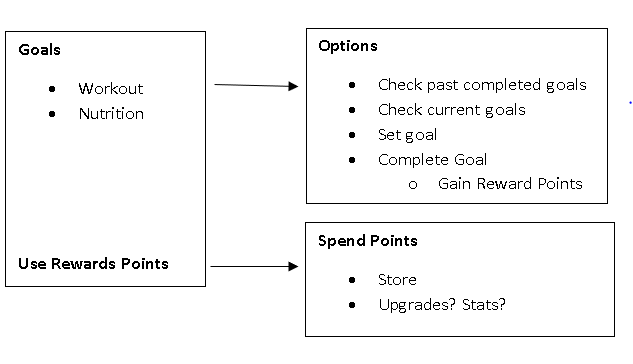
\includegraphics[width = 15cm, height=9cm]{Diagram}

\noindent The diagram above shows an outline of the program we are making.  The main features that we want to approach first are shown here.  These features include setting goals, completing goals, checking current and past goals, and using reward points from the completed goals to get in-game rewards from the store.


\subsection{Useful Programming Languages and tools used for this project}
The programming languages and tools that will be used in the project are HTML, CSS, JavaScript, Ruby on Rails, Bootstrap and GitHub.  We discerned that making a web application will be the easiest way to approach this program, so HTML, CSS, and JavaScript are the most appropriate programming languages for this project.  Ruby on Rails and Bootstrap a free open source software that is designed for modern web applications, making them appropriate tools for this project.  Github will be used to help organize everything and allow members to access the files within the project.

\subsection{What are the functional requirements?}
Our web application needs to be mobile friendly, it will set a goal list, that is modifiable by the user, and that give points or rewards when the user accomplish one action in the list, such as running one mile.\newline

\noindent It will also require input of weight, height, gender, age and activity level for the nutrition feature of the app, then the program will provide output accordingly.


\subsection{What are its non-functional requirements?}
The web app should be able to accept upgrades, accomplished goals should be stored into the history option of the app.


\subsection{What other documentations will we provide to help our users understand and use our system?}
There will be no outside documentations to help users understand our system.  There will be a help button that will describe what actions can be done in the application, and what they do.  We are potentially thinking of implementing a tutorial, but we believe a help button will suffice.

\subsection{What are the major features of the system that make it so effective and useful?}
The major features of the application include the ability to set workout and nutrition goals, and the ability to track the progress of the user.  These features will help users obtain a healthier lifestyle and is effective due to the reward system that will motivate users.  We are tentative on including a Gym Pal system which will help users find partners for their workouts.  While this is another motivation for users to stay healthy, we want to focus more on personal goals and workouts for the user. 

\section{Use Cases}
A user can be looking to become more healthy by setting healthy goals. How does a person accomplish these goals. By setting goals on our online application, users are rewarded for accomplishing workouts. Consistency is key to accomplish any difficult task. Working out is a difficult task. So why not make working out fun? 
\newline
\newline
Flow of events:
\begin{itemize}
\item Main menu displays Goals, Nutrition, Workout Bud, and Store
\item To set a goal, user selects goals
\item Win points for accomplishing goal
\item Spend points from accomplishing goals
\item Acquire more in-store items by setting more goals 
\item View history of accomplishments 
\item Personally benefit from making healthy lifestyle choices!
\end{itemize}
Quality Requirements:
\newline

\begin{itemize}
\item Access to our online web application via computer, phone, tablet
\item To accomplish goals the user will enter in data from their accomplishments(runs, workouts, etc.). 
\end{itemize}

\graphicspath{ {files/graph.png} }
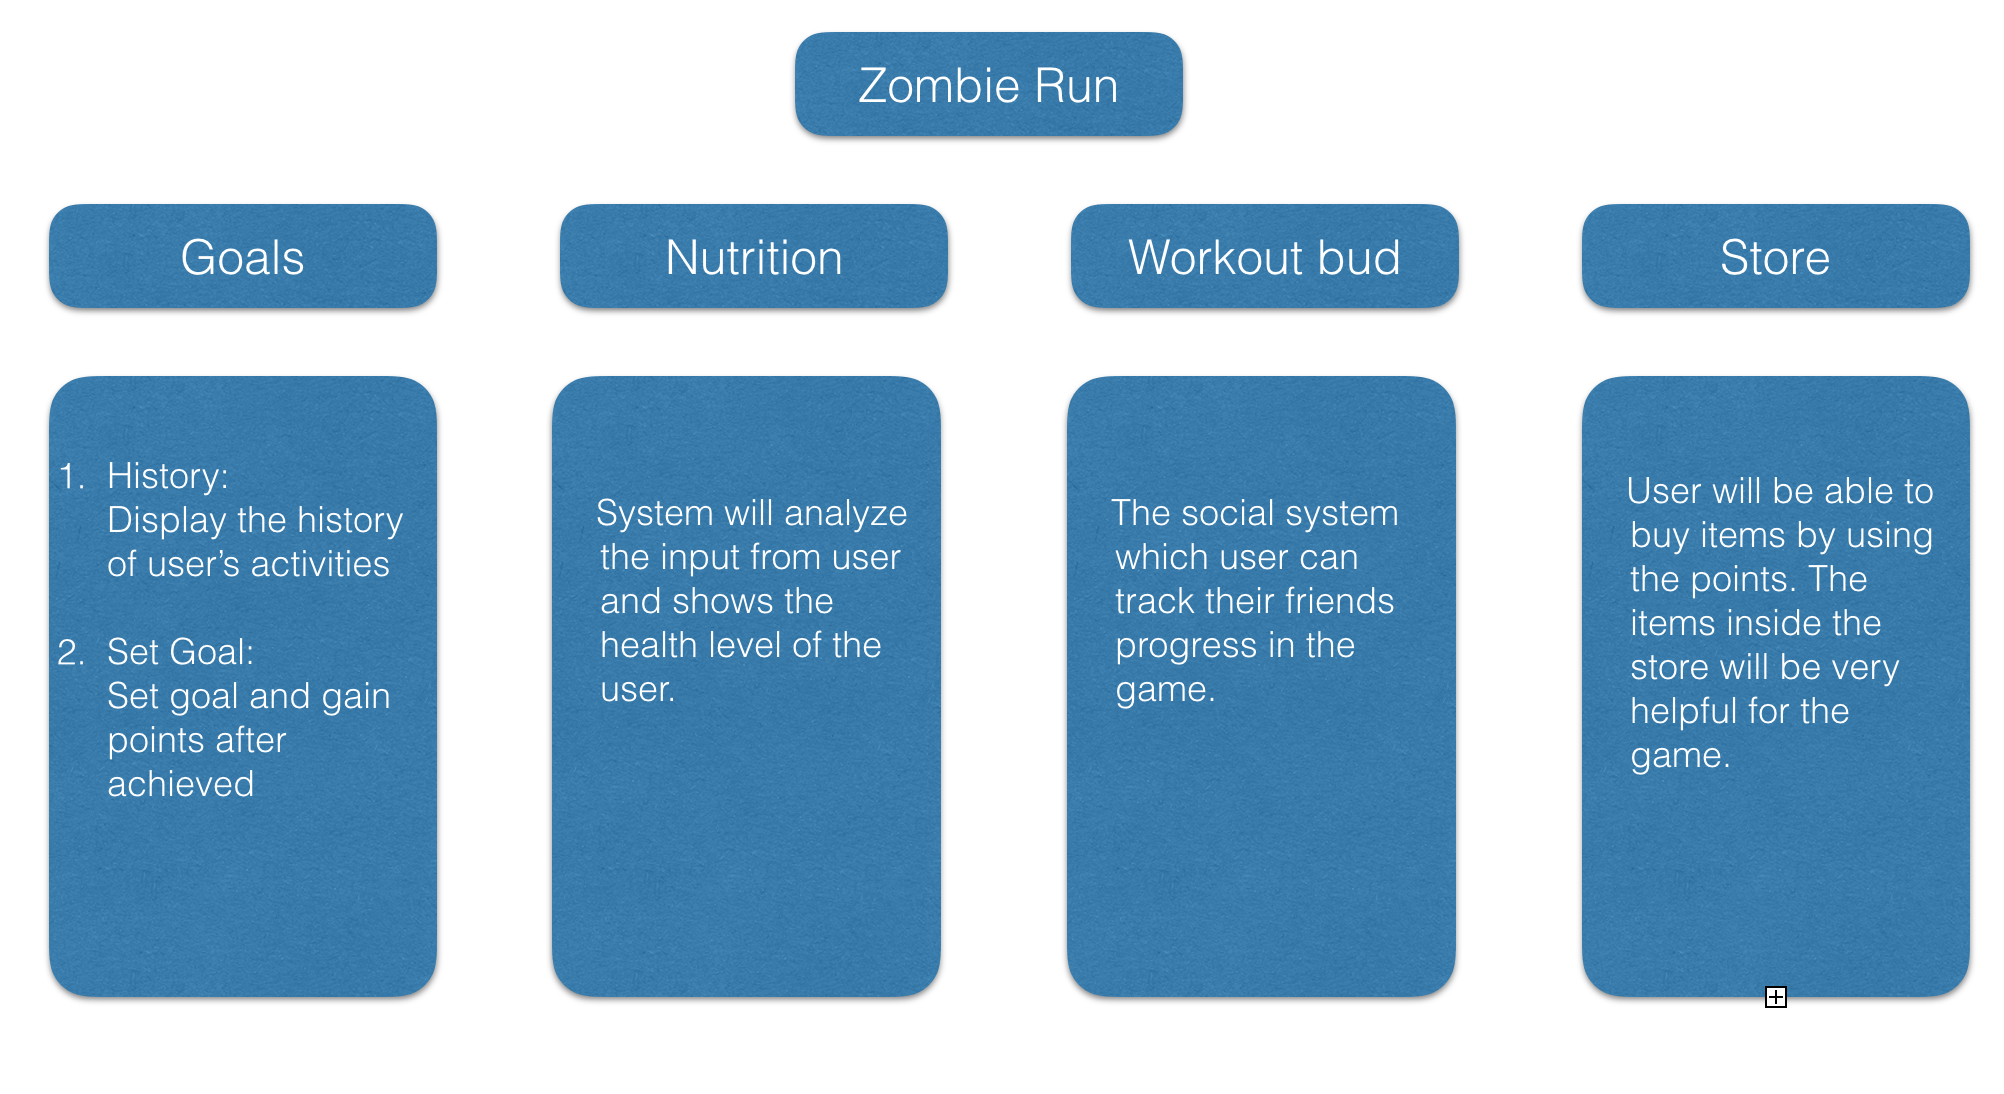
\includegraphics[width = 15cm, height=10cm]{graph}

\subsection{Scenario 1:}
Name: Setting a workout and nutritional goal\newline
\\
Goal Level: Allow the user to set physical  or nutritional goals for themselves that will produce rewards when completed.\newline
\\
Actor: Application user.\newline
\\
Preconditions:
\begin{itemize}
\item User uses/clicks the "set goal" option
\item A goal is now created and the user can work to finish it
\end{itemize}
Postconditions:
\begin{itemize}
\item Once the user finishes the goal, they enter the information from their goal. This can be the number of miles ran or number of push ups
\item The goal will be recorded and can be checked by the user.
\item the user will be rewarded for achieving the goal by points
\item A reward will be generated and listed on the goal set by the user.  This reward will be given when the user completes the goal.
\end{itemize}


\subsection{Scenario 2:}
Name: Check History\newline
\\
Goal: Allows the user to check a list of past goals that have been completed by the user.\newline
\\
Actors: Application user\newline
\\
Precondition: 
\begin{itemize}
\item The user uses/clicks the "Goals" option, then "history"
\end{itemize}
Postcondition: 
\begin{itemize}
\item A list of past activities
\item The user now can create new goals based off of past activities
\end{itemize}



\subsection{Scenario 3:}
Name: Store \newline
\\
Goal: Users will be able to purchase items by using the points they have earned. The items inside the store will increase the survival rate of the user.\newline
\\
Preconditions:
\begin{itemize}
\item User selects store
\item User purchases a item from the in game store
\item User attempts to purchase another item they do not have enough points for
\end{itemize}
Postcondition:
\begin{itemize}
\item User can use the items they bought
\item User is alerted that they do not have enough coin and must set more goals for more rewards
\end{itemize}

\subsection{Why these scenarios are helpful}
The three scenarios are the most important because they discuss how the user used different core parts of our application. Goal setting is our primary objective for users to begin doing for themselves in their every day lives. \newline
\\ Scenario 1 describes the actor setting a workout and nutritional goal. The workout and nutritional goals themselves are separate options within the main user interface. Once the actor selects either goal it is up to them to complete their goal. Whether it is to go on a 2 mile run, or 100 push ups, or eating nutritionally healthy. When the user finishes their goal, they enter in the data from the workout and then they are rewarded points! \newline
\\ Scenario 2 describes how the user can view their recent goals. By viewing recent goals, this will help users create new goals to be achieved.\newline 
\\ Scenario 3 describes the actor utilizing our in game store! In this scenario, the user buys an item from our in game store. The purchase was successful and the reward was awesome! But, the actor or user, ran into a situation where they don't have enough points to purchase an item. They must accomplish more goals in order to acquire more points and in return, purchase more rewards! 

\subsection{Error Scenarios}
Since the premise of our game is based on users setting their own goals. Then the user enters their own data such as how many miles they ran. So the honor system will be upheld to our users. Potentially our users can just sit on the couch and enter in that they went on a 50 mile run. A few ways around this is by setting limits on the data users enter and how often they are able to enter in new goals. 

\section{Planning}
\subsection{Milestones \& Tasks}

To begin building the Zombie Apocalypse Prep App, we will split the project into the three key features; GitFit, Nom and GymPal. Before beginning development, we will ensure each individual has the correct environment setup for development.\newline

\noindent The first feature is the most important to the development of the app would be GitFit. This would require an option for a goal to be generated, and when the goal is completed, or checked off an arbitrary amount of points are rewarded, and added to whatever number is currently awarded. Ideally the goal will be customizable. The interface will need to be 'lightly' developed to allow a goal to be made, and removed upon completion.\newline

\noindent The second feature, seems straightforward to program. It would rely on the user entering numeric information about themselves, and the program would generate nutritional recommendations to them, such as height and weight. It would be based on an equation that takes the user's h The program would suggest how much protein, fat, and carbohydrates the user ought to eat each day. A forum would need to be written to allow the user to input the information, and background logic would be used. Lastly, a table would need to written with the correct information displayed.\newline

\noindent The last feature, GymPal, would require accounts to be made for users to communicate in a forum. The system would rely on Ruby on Rails to create accounts, and allow users to create posts and comments. \newline

\subsection{Schedule and Timeline} 

\graphicspath{ {files/Capture.png} }
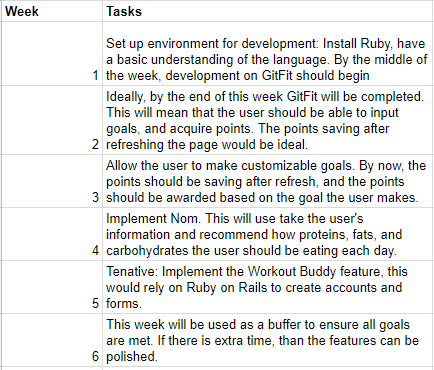
\includegraphics[width = 15cm, height=10cm]{Capture}\\ 

\noindent To begin building the Zombie Apocalypse Prep App, we will split the project into the three key features; GitFit, Nom and GymPal. Before beginning development, we will ensure each individual has the correct environment setup for development.\newline

\noindent The first feature is the most important to the development of the app would be GitFit. This would require an option for a goal to be generated, and when the goal is completed, or checked off an arbitrary amount of points are rewarded, and added to whatever number is currently awarded. Ideally the goal will be customizable. The interface will need to be 'lightly' developed to allow a goal to be made, and removed upon completion.\newline

\noindent The second feature, Nom seems straightforward to program. It would rely on the user entering numeric information about themselves, and the program would generate nutritional recommendations to them, such as height and weight. It would be based on an equation that takes the user's h The program would suggest how much protein, fat, and carbohydrates the user ought to eat each day. A forum would need to be written to allow the user to input the information, and background logic would be used. Lastly, a table would need to written with the correct information displayed.\newline

\noindent The last feature, GymPal, would require accounts to be made for users to communicate in a forum. The system would rely on Ruby on Rails to create accounts, and allow users to create posts and comments. 


\subsection{Project tracking} 

We will use GitHub to monitor the progress of the app. By using GitHub we can track who did what, and when. Additionally, by using GitHub we can ensure that there is a history of the code as the project grows, allowing us to take steps back if needed. To ensure the quality of our work, we'll operate on a pull request/merge system; that is, when a branch is ready to be merged with the master branch, a pull request will be made and the code will be reviewed. Furthermore, if a goal isn't met, we will begin working together to meet the goal of that specific feature. To track what needs to be done, Github Issues will be made, and we can self-assign ourselves on what interests us, or what needs to be done. When the Issue is completed, it will be completed in the pull request section of GitHub.\newline

\noindent To ensure goals are met the group will not move on to the next feature until the current feature is implemented fully, and doesn't cause conflicting problems with another feature.

\subsection{Risk Management} 

Risk 1: Team Collaboration using Git may become a risk.\newline
Likelihood of risk: Medium probability \newline
Impact to project: Bad Github practice can lead to deletion or unwanted Modification in the project source code.\newline
Address risks: To prevent this risks to occur, a good and clean work-flow structure need to be determined before any submission takes place and is expected that each developer uses its own branch to make changes to the root project.\newline

\noindent Risk 2: Problems using Ruby on Rails \newline
Likelihood of risk: Medium probability\newline
Impact to project: If a good working comprehension of ruby is not accomplished, bugs and other undesirable outputs can affect the application functionality.\newline 
Address risk: To prevent risks related to bad ruby on Rails practice we will meet weekly to address the learning advances of each team member in relation of this language.\newline

\noindent Risk 3: Scope Creep\newline
Likelihood: Mid to hight \newline
Impact to project: If new, not previously planned features are added to the application, we may have functionality problems, that can lead to the application not working or working incorrectly.\newline 
Address risk: To prevent non planned features to be added is important to follow a group work-flow system and report our advances each week.

\section{Meeting Report}

\subsection{Progress Made} 
The team members working on the Zombie Apocalypse Prep App came together this week to introduce each other and get to know each person strengths and weaknesses in relationship to software engineering and programming in general.\\ We discussed how to approach the front and back end of the project, we also created a developing plan, and with a schedule to establish when is the most convenient time to meet for each member of the team.
Additionally, we developed milestones to follow during the developing cycle, and established the goals for next week.
\\
\subsection{Next Week Goals} 
The general goal for next week is to create a baseline framework for the application. The framework will be pushed into our group github repository for further modifications.\\ The other goal is for the members that haven't used Ruby on Rails to download and become familiar with the software. The members will accomplish becoming familiar with the software by reading an online tutorial supplied by a on line textbook[1]. YouTube and similar platforms will also be used for extended research. 
\\
\subsection{Contributions} 
All members working on the project contributed to the writing of this Latex document, Eric Sisson did the diagram that addresses how our approach plugs into existing resources, Kuan-Yu Lai made the use case diagram,, Christa Wright create the Schedule and Timeline section of the document and Jorge Guzman Nader wrote the meeting report and Project description section.\\ All members also help to set the scheduling of future meetings, the establishment of milestones for the project and the goals to be accomplished in a given timeframe.\\ For future reference, the group will use Github as our main contribution platform, in which is expected of each member to work in a section of the code.
\\
\subsection{Customer} 
We meet with our costumer, and started to brain storm about the front-end phase of the web application, and how the main menu will look and act.\\ A diagram about tentative functionalities for the app was made, and some of the sub-field of the app were either introduced or discarded based on resources capabilities and time constrains. 
\\
\section{Citations: }
[1] https://www.railstutorial.org/book~\cite{web1}\newline
[2]	https://www.w3schools.com/~\cite{web2}\newline 
[3] https://github.com/~\cite{web3}\newline
[4] http://www.beyondorganic.net/dri-calculator.html~\cite{web4}\newline
[5] http://getbootstrap.com/~\cite{web5}\newline
\end{document}